\documentclass[12pt, a4paper]{article}
\usepackage[utf8]{inputenc}
\usepackage[english]{babel}
\usepackage{fancyhdr}
\usepackage{framed}
\usepackage[dvipsnames]{xcolor}
\usepackage{tcolorbox}
\usepackage{graphicx}

\title{Introduction to Permutation and Combination}
\author{SM}
\date{2022}

\pagestyle{fancy}
\fancyhf{}
\rhead{SM}
\lhead{Permutations and Combinations}
\rfoot{Page {\thepage}}

\begin{document}

\maketitle
\newpage
\tableofcontents
\newpage

\section{Introduction}
\subsection{Fundamental Principle of Counting}
\begin{tcolorbox}[colback=TealBlue!10!White,colframe=TealBlue!50!black]
\textbf{Addition Rule:} If an event can occur through a process m ways or with another process in n ways, then the total number of ways with which the event can occur is m+n. The processes here must be mutually exclusive.\newline
\textbf{Multiplication Rule:} If an event can occur in m ways, and another event can occur in n ways, then total number of ways in which both event can occur simultaneously is m×n. Ensure while using this rule, that the events are independent.
\end{tcolorbox}
\textbf{NOTE:} See that, how the words `and', `or' are used while defining the rules. These rules can be extended for more events as well.\newline

\textbf{Example 1:} Suppose you can reach a certain destination A from your starting point, using 3 different trains or 2 different buses. What are the total number of ways by which you can reach A?

\textbf{Solution} Here it is simple that, you can either use the trains, or you can use the buses. So the total number of ways to reach A is 2+3 = 5

\textbf{Example 2:} In continuation of the last example, suppose yo have to reach, another destination B from A, such that you can use 2 different trains or 4 different buses. What are the total number of ways you have in order to reach B from your starting destination?

\textbf{Solution} In the last example, we have found that there are 5 ways to reach A, and now for moving from A to B we have 2+4 = 6 ways. Since, the mode of transport we use from A to B is independent of the mode of transport we use from starting destination to A, the total number of ways we have to reach B from our starting destination is 5 × 6 = 30 ways.\newline \newline 
For moving further, we must be knowing some other basic concepts which will be listed as follows:
\begin{itemize}
    \item \textbf{Factorial Notations:} If n is a positive integer, n factorial is defined by n! = 1×2×3×4....×n i.e. 2! = 1×2 and 3! = 1×3 , however there is a special case, 0! = 1.
    \item Number of favourable results = Total number of results - number of unfavourable results
\end{itemize}

\newpage
\subsection{Some examples based on fundamental rules}
\textbf{Example 3:} If a coin is tossed twice, find total number of outcomes.

\textbf{Solution} Tossing of a coin can either result in a head of a tail, giving two outcomes for each toss. If it is tossed twice, it can give a total of 2×2 = 4 outcomes. To understand this we can list out the outcomes as {(H,T),(H,H),(T,H),(T,T)}.\newline
\textbf{Example 4:} Find the number of ways in which three out 7 different books can be placed on a shelf.

\textbf{Solution} In the first place, we can place any 1 out of 7 books. So number of ways to fill first place is 7. For second place, we have 6 books remaining, so number of ways to fill second place is 6, and proceeding the same way, for the third place number of ways is 5. So the total number of ways: 7×6×5 = 210. (We will not do 7+6+5 here because we are asked to fill all the spaces simultaneously. We cannot fill any one of first or second or third place)\newline
\textbf{Example 5:} Find the number of ways to arrange 7 different pens on 7 pen holders, each one containing only one pen.

\textbf{Solution} Proceeding the same way as in example 4, for first place number of ways are 7, for second place it's 6, followed by 5,4,3,2,1 for third, fourth, fifth and sixth place. Hence answer will be = 7×6×5×4×3×2×1 = 7! = 5040 \newline
\begin{tcolorbox}[colback=TealBlue!10!White,colframe=TealBlue!50!black]
\textbf{Arranging n-distinct objects}
From examples 4 and 5, we can understand that n-different objects can be arranged in n! ways
\end{tcolorbox}

\section {Permutation and Combination}
\begin{tcolorbox}[colback=TealBlue!10!White,colframe=TealBlue!50!black]
We have the general formula, which states number of ways in which r objects can be selected out of n-distinct objects = $^{n}C_{r} = \frac{n!}{r!(n-r)!}$. This can also be stated as, combination of n objects taken r at a time. \newline
Number of permutations of n different objects taken r at a time is given as $^nP_r$ = $^{n}C_{r}.(r!)$ = $\frac{n!}{(n-r)!}$
\end{tcolorbox}[colback=TealBlue!10!White,colframe=TealBlue!50!black] 
Here, we see that n and r are number of objects, so they have to be positive integers with $n \geq r$.\newline \newline
\textbf{Explaining the formula for permutations and combinations}:
Let us say, we have n objects but only r places and each place can accommodate only 1 object. This means, the first place can be filled in $n$ ways, the second in $n-1$ ways the third in $n-2$ ways and so on until the rth place which can be filled in $n-r+1$ ways. We have now, number of ways = $n(n-1)(n-2)....(n-r+1)$. In factorial notation, this can be expressed as $\frac{n!}{(n-r)!}$. This is the formula for number of permutations of n objects taken r at a time, and is denoted as $^nP_r$ or $_nP_r$. Note, that here we did place objects in different spaces available right from the first place, that is, it is ordered arrangement. When order is immaterial, it is referred to as combination which is denoted as $^nC_r$ or $_nC_r$ and can be given as $^nC_r$ = $\frac{n!}{(n-r)! r!}$. \newline The following examples will help in understanding the difference between a permutation and a combination.\newline
\textbf{Example 6:} In how many ways can we select 3 objects out of 7 different objects?

\textbf{Solution} Here, we have to select objects, order is immaterial, so we use the formula for combination of n different objects taken r at a time which gives, $^7C_3$ = 35.\newline
\textbf{Example 7:} Find number of arrangements of 7 different objects taken 3 at a time.

\textbf{Solution} Suppose we choose, the different objects A,B,C. Then in terms of arrangements, ABC and ACB are two different arrangements. Here, it is an ordered arrangement. We use the formula for permutation of n different objects taken r at a time which gives, $^7P_3$ = $^7C_3.(3!)$ = 210.\newline
\textbf{Example 8:} How many triangles can be made by joining vertices of a hexagon?

\textbf{Solution} For a triangle, we need to choose three vertices out of the six vertices of the hexagon. Hence number of triangles = $^6C_3$ \newline
\textbf{Example 9:} A committee of 6 members is to be made from 5 women and 5 men such that exactly 3 men and 3 women are selected. Find the number of such committees that can be formed.

\textbf{Solution} We can select 3 men out of 5 in $^5C_3$ ways and similarly $^5C_3$ ways for selecting 3 out of 5 women. Since selection of men and women are independent, total number of teams that can be made is $^{5}C_{3} \times ^{5}C_{3} = 100$.
\section{Circular Permutations}
Till now, we have discussed about linear permutations. Now, we talk about arrangements in circular manner. Consider three persons- A, B and C. In linear permutations the arrangement $ABC$ and $CAB$ are two different arrangements, while in circular permutation, both are same. In figure 1, we place both $ABC$ and $CAB$ in circular manner. Now, in the left diagram, looking from $A$'s perspective, the person on its right is $C$ and on the left is $B$. Now again in the right diagram, the position of $B$ and $C$ did not change with respect to $A$. This can be observed that the diagram in the right is obtained by rotating the one in the left. In circular permutations, arrangements produced by such rotations are considered identical.
\begin{figure}
    \centering
    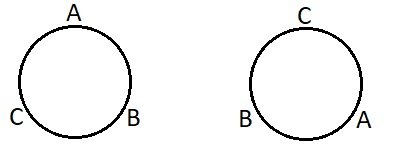
\includegraphics[width=7cm]{PnCcircularpermu.jpg}
    \caption{The left one shows ABC(clockwise), right one shows CAB(clockwise)}
    \label{fig:my_label}
\end{figure} \newline
Now we think of $N$ such objects to be placed in $N$ place where each place accommodates only one object (circular permutation). Let us now call them object $A_{1}$, $A_{2}$, $A_3$ ...$A_n$. Once we fix any of these, say $A_1$ in the next position (in clockwise direction) $n-1$ objects can be placed, followed by $n-2$ objects for the next place and so on until there is just one last position remaining completing the circle. From the above discussion we get that total number of such permutations will be $(n-1)(n-2)(n-3)(n-4)$...$1$ = $(n-1)!$ 
\begin{tcolorbox}[colback=TealBlue!10!White,colframe=TealBlue!50!black]
The total number of circular permutations of n-objects is $(n-1)!$.
\end{tcolorbox}
\textbf{Example 10:} Find the total number of ways in which 7 children can be seated in a round table for community lunch.

\textbf{Solution} Total number of ways will be = (7-1)! = 6!\newline
\textbf{Example 11:} A person is to make a garland with 6 different flowers. Find the total number of possible arrangements of flowers in garland.

\textbf{Solution} Here, the sense of clockwise and anticlockwise makes no difference, as the garland can be turned around. Hence the total number of possible arrangements = $\frac{(6-1)!}{2}$ = $\frac{5!}{2}$
\section{Tie and Gap Method}
\begin{tcolorbox}[colback=TealBlue!10!White,colframe=TealBlue!50!black]
\textbf{Tie method:} If r objects out of n objects should always be together in different arrangements, then total number of permutations in such case is $(n-r+1)!(r!)$
\end{tcolorbox}
Let us understand this using the following example:\newline
\textbf{Example 12:} Find the total number of ways of forming a queue of 11 students of a class where 4 students always stand consecutively.

\textbf{Solution} Since 4 students have to be together, we first consider them as 1 unit (tie them) permute this unit with rest of the students and then finally permute the 4 students among themselves which gives the answer $8! \times 4!$.
\begin{tcolorbox}[colback=TealBlue!10!White,colframe=TealBlue!50!black]
\textbf{Gap method:} If no two of some objects should be placed together (in permutation) then excluding them, permute rest and in created gaps, permute those objects.
\end{tcolorbox}
\textbf{Example 13:} Find the total number of ways for 8 people to stand in a row, of which two particular persons $A$ and $B$ do not stand together.

\textbf{Solution} First, we permute the rest 6 people and in the created 7 gaps (starting from the left of first person to the right of last person), we choose any two gaps where we can place $A$ and $B$ and we also keep in mind, that $A$ and $B$ can permute among themselves. Hence the answer becomes $6! \times {^7C_2}\times 2!$
\section{Permutation of alike objects(all at a time)}
\begin{tcolorbox}[colback=TealBlue!10!White,colframe=TealBlue!50!black]
Let out of n objects, $n_1$ are alike objects of one kind, $n_2$ are alike objects of other kind .... $n_k$ are alike objects of another kind and remaining are different, then number of permutation of these n objects taken all at a time is $\frac{n!}{(n_{1}!)(n_{2}!)...(n_{k}!)}$.
\end{tcolorbox}
To understand this formula, let us take the example of arranging the letters of the word $PERMUTATION$. Here the two $T$'s are identical. Rest all letters are different. Now, suppose we are to permute the letters of this word. How many such permutations are possible?

Suppose we name the two $T$'s as $T_1$ and $T_2$ which gives $11!$ permutations of the word. Now, consider two words from these permutations, say, $PERUMT_{1}AT_{2}ION$ and $PERUMT_{2}AT_{1}ION$. Had the $T$'s not been numbered, a person would have read $PERUMTATION$ in both the cases and will not identify the two cases as different arrangements. So the total number of permuations will become $\frac{11!}{2!}$.\newline
\textbf{Example 14:} Find the number of ways of arranging the letters of the word $HANNAH$.

\textbf{Solution} Here we see, that we are given with 2 $H$'s, 2 $N$'s and 2 $A$'s. Now consider the two $H$'s being $H_1$ and $H_2$, the two $N$'s being $N_1$ and $N_2$ and the two $A$'s being $A_1$ and $A_2$. Now consider a permutation of this word, say, $N_{1}A_{1}H_{1}H_{2}A_{2}N_{2}$. Interchanging any of the repeated letters gives a new permutation but in original question the letters are not numbered, which means that interchanging the identical letters gives no new permutation.\newline
\textbf{Example 15:} Find the total number of possible arrangements of the letters of the word $MISSISSIPPI$ such that now two $I$ are together.

\textbf{Solution} Here, first we separate out 4 $I$'s and permute the remaining seven letters which can be done in $\frac{7!}{4!2!}$. The $4!2!$ in the denominator is due to the repeated letters $S$ and $P$. Now out of the 8 created gaps we select 4 gaps in $^8C_4$ ways. Hence the answer becomes $\frac{7!}{4!2!}{^8C_4}$. \newline
\textbf{Example 16:} Find the total number of possible arrangements of the letters of the word $MISSISSIPPI$ such that all $S$'s are not present together.

\textbf{Solution} We are asked to find the arrangements where all the $S$ are not present together, which means that atmost three $S$ can be present together. There are two methods to do this problem. First one, where we can make cases representing no two $S$ together, only two $S$ together and three $S$ together and then add them. The second and the easier way will be to use bijection rule. We will first calculated the number of all possible arrangements of the letters of the word $MISSIPPI$ without any restriction and then we will subtract the number of cases where all the $S$ are together.
\begin{center}
 Hence, required answer = (number of all possible arrangements) $-$ (number of arrangements where all $S$ are together) \newline = $\frac{11!}{4!4!2!}$ $-$ $\frac{8!}{4!2!}$
\end{center}

   
  



\end{document}